\section{Conditional Expectation}

  Conditional expectation is extremely important, especially in the context of stochastic processes, which is talked about in more detail in another set of notes. 

  First, note that when we talk about the probability of event $A$ happening, or equivalently, the probability of $\omega \in A$, we can write this as the expected value of the indicator function $A$. 
  \begin{equation}
    \mathbb{P}(A) = \mathbb{E}[1_A]
  \end{equation}
  This will come in handy later in connecting conditional probability and expectation. 

  Now conditional expectation is quite tricky to understand at first. We will start by defining it given a $\sigma$-algebra and then given a \hyperref[def:random-variable]{random variable}. 

  \begin{definition}[Conditional Expectation]
    \label{def:cond-exp}
    Given a \hyperref[def:probability-space]{probability space} $(\Omega, \mathcal{F}, \mathbb{P})$, a sub-$\sigma$-algebra $\mathcal{G} \subset \mathcal{F}$, and an $\mathcal{F}$-measurable \hyperref[def:random-variable]{random variable} $X$ (with $\mathbb{E}[X] < \infty$), the \textbf{conditional expectation of $X$ given $\mathcal{G}$} is defined to be the $\mathcal{G}$-measurable random variable $Y = \mathbb{E}[X \mid \mathcal{G}]$ satisfying 
    \begin{equation}
      \int_A X \,d\mathbb{P} = \int_A Y \,d \mathbb{P}
    \end{equation}
    or equivalently, 
    \begin{equation}
      \mathbb{E}[X \cdot 1_A] = \mathbb{E}[Y \cdot 1_A]
    \end{equation}
    for all $A \in \mathcal{G}$. Any $Y$ satisfying these two conditions is said to be a \textbf{version} of $\mathbb{E}[X \mid \mathcal{F}]$. The critical detail to note here is that the conditional expectation $Y$, has the same expected value as $X$ does, not over just the whole $\mathcal{G}$, but \textit{in every subset $G$ of $\mathcal{G}$}. 
  \end{definition}
	\begin{proof}
		We should claim that it always exists and it is unique up to measure $0$. 
		\begin{enumerate}
			\item \textit{Uniqueness} Show that if $Y$ is a version, then $\mathbb{E}[|Y|] < +\infty$. Hint: Show that $\mathbb{E}[|Y|] < \mathbb{E}[|X|]$. We split $Y = Y+ - Y_{-}$. Then, $\mathbb{E}[|Y|] = \mathbb{E}[Y_+] + \mathbb{E}[Y_-]$, and we can bound 
				\begin{align}
					\mathbb{E}[Y_+] = \int_{\mathbb{R}_{>0}} Y_+ \,d\mathbb{P} = \int_{\mathbb{R}_{>0}} X \,d\mathbb{P} \leq \int_{\mathbb{R}_{\geq 0}} |X| \,d\mathbb{P} \\ 
					\mathbb{E}[Y_-] = \int_{\mathbb{R}_{<0}} Y_- \,d\mathbb{P} = \int_{\mathbb{R}_{<0}} X \,d\mathbb{P} \leq \int_{\mathbb{R}_{< 0}} |X| \,d\mathbb{P} 
				\end{align}
				Combining these together, we get $\mathbb{E}[|Y|] < \mathbb{E}[|X|]$. To prove uniqueness, we can see that if $Y, Y^\prime$ are two versions of $\mathbb{E}[X \mid \mathscr{F}]$, then let $A_\epsilon = \{\omega \in \Omega \colon Y(\omega) - Y^\prime (\omega) > \epsilon \}$. Then, 
				\begin{equation}
					\mathbb{P}(A) \epsilon \leq \int_A (Y - Y^\prime) \,d\mathbb{P} = \int_A (X - X) = 0 \implies Y \leq Y^\prime \text{ a.s.}
				\end{equation}
				Now swap $Y$ and $Y^\prime$ to get $Y^\prime \leq Y$. 
			\item \textit{Existence}. To prove existence of $Y$, this is much more involved. Recall the definition of \hyperref[mt-def:absolutely-continuous-measures]{absolutely continuous measures} and $\sigma$-finite measures, along with the \hyperref[mt-thm:rn-der]{Radon-Nikodym theorem}. We will use this to construct our \hyperref[def:cond-exp]{conditional expectation}. Since we can write $X = X_+ - X_-$, WLOG let $X \geq 0$. Let $\mu = \mathbb{P}$, we are looking for $Y$ s.t. for all $A \in \mathscr{F} \subset \mathscr{F}_0$, 
				\begin{equation}
				  \int_A Y \,d\mu = \int_A X \,d\mu
				\end{equation}
				Now set $\nu(A) \coloneqq \int_A X \,d\mu$, which turns out to be a $\sigma$-finite measure on $(\Omega, \mathscr{F})$. By construction, $\nu << \mu$. By the Radon-Nikodym theorem, $\exists f$ s.t. for all $A \in \mathscr{F}$, 
				\begin{equation}
				  \int_A f \,d\mu = \nu(A) = \int_A X \,d\mu
				\end{equation}
				Now set $f = Y$. 
		\end{enumerate}
	\end{proof}

	For now, we can interpret this as the best approximation of the $\mathcal{F}$-measurable $X$ with the $\mathcal{G}$-measurable $Y$. Here is a useful analogy. Say that we have some "fine" function $X$ defined on the interval $[0, 1]$ with a fine Borel $\sigma$-algebra $\mathcal{F}$. 
  \begin{enumerate}
    \item If we are given some sub-$\sigma$-algebra $\mathcal{G}$ composed of $\emptyset, [0, 0.5], (0.5, 1], [0, 1]$, then $Y$ would be the step function defined constantly on these intervals. 
    \item If we are given a finer sub-$\sigma$-algebra $\mathcal{H}$ generated by $[0, 0.25), [0.25, 0.5), [0.5, 0.75), [0.75, 1]$, then this would give a $\mathcal{H}$-measurable function that is a better approximation of $X$. 
  \end{enumerate}
  \begin{center}
    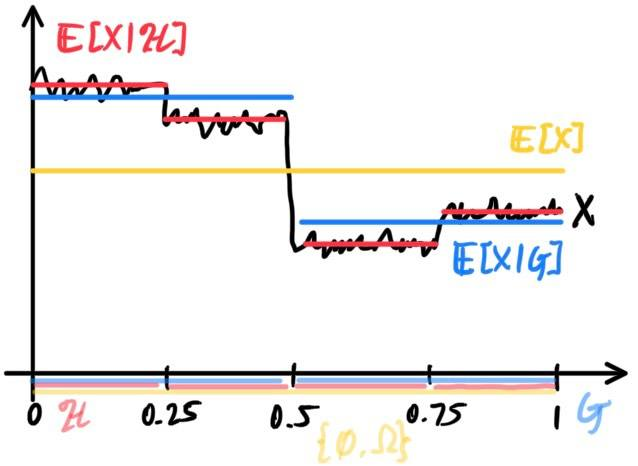
\includegraphics[scale=0.33]{img/function_approximation_conditional.jpg}
  \end{center}

  Therefore, we can see that if $\mathbb{E}[X \mid \mathcal{G}]$ is $\mathcal{F}$-measurable, then 
  \begin{equation}
    X = \mathbb{E}[X \mid \mathcal{G}]
  \end{equation}
  since its value coincides with $X$ for every event in $\mathcal{F}$. One way to think about it is that $\mathbb{E}[X \mid \mathcal{G}]$ is the \hyperref[def:cond-exp]{conditional expectation} of $X$ (which is "detailed" up to resolution $\sigma(\mathcal{G})$) taken with a camera of resolution $\mathcal{G}$. The finer (bigger) the $\sigma$-algebra is, the higher the resolution. 

	\begin{example}[Conditional Expectation from a Joint Density]
	  \label{ex:conditional-expectation-from-a-joint-density}
		Suppose $X, Z$ are \hyperref[def:random-variable]{random variables} with a joint pdf $f_{X, Z} (x, z)$ and $\mathbb{E}[|X|] < +\infty$. Then, we define the conditional pdf as 
		\begin{equation}
			f_{X\mid Z} (x \mid z) \coloneqq \begin{cases} 
				\frac{f_{X, Z} (x, z)}{f_Z (z)} & \text{ if } f_Z (z) \neq 0 \\  
				0 & \text{ if } f_Z (z) = 0 
			\end{cases}
		\end{equation}
		Define $Y(z) \coloneqq \int_{\mathbb{R}} x f_{X \mid Z} (x \mid z) \,dx$. We claim that $Y(Z)$ is a version of $\mathbb{E}[X \mid \sigma(Z)]$. As a proof, for all $A \in \sigma(Z)$, we have 
		\begin{align}
			\int_A Y(z) f_Z (z) \,dz & = \int_A \bigg( \int_{\mathbb{R}} x f_{X \mid Z} (x \mid z) \,dx \bigg) f_Z (z) \,dz \\ 
															 & = \int_A \int_{\mathbb{R}} x f_{X, Z} (x, z)\,dx\,dz
		\end{align}
		where we denote $dx, dz$ are the Lebesgue or counting measure, depending on whether it is discrete or continuous. 
	\end{example}

	\begin{theorem}[Linearity]
	  \label{thm:linearity}
	  We have 
		\begin{equation}
			\mathbb{E}[a X_1 + b X_2 \mid \mathscr{G}] = a \mathbb{E}[X_1 \mid \mathscr{G}] + b \mathbb{E}[X_2 \mid \mathscr{G}]
		\end{equation}
	\end{theorem}
	\begin{proof}
	  We use linearity of the integral. For all $A \in \mathscr{G}$, 
		\begin{equation}
			\int_A (a X_1 + b X_2) \,d\mathbb{P} = a \int_A X_1 \,d\mathbb{P} + b \int_A X_2 \,d\mathbb{P} = a \int_A \mathbb{E}[X_1 \mid \mathscr{G}] \,d\mathbb{P} + b \int_A \mathbb{E}[X_2 \mid \mathscr{G}] \,d\mathbb{P}
		\end{equation}
	\end{proof}

  \begin{theorem}[Conditional Expectation as Orthogonal Projection]
    \label{thm:conditional-expectation-as-orthogonal-projection}
    Suppose $\mathbb{E}[X^2] < \infty$. Then, $\mathbb{E}[X \mid \mathcal{G}]$ is the $\mathcal{G}$-measurable function $Y$ that minimizes the mean squared error 
    \begin{equation}
      \mathbb{E}[ (X - Y)^2]
    \end{equation}

    \begin{figure}[H]
      \centering 
      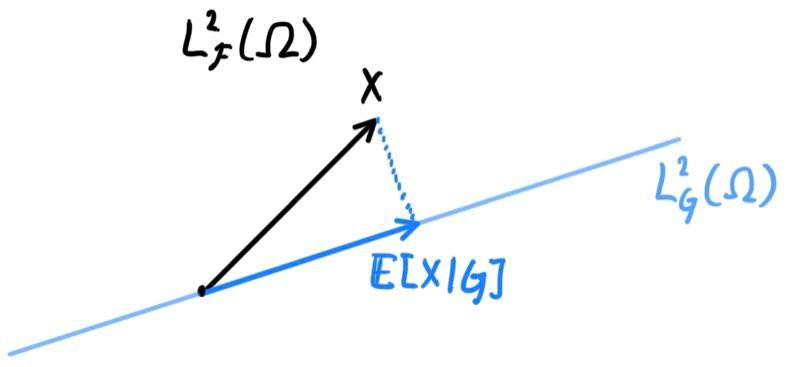
\includegraphics[scale=0.3]{img/Hilbert_Space_projection.jpg}
      \caption{This gives a nice geometric interpretation of $\mathbb{E}[X \mid \mathcal{G}]$. Given that $X$ lives in the Hilbert space $L^2_\mathcal{F} (\Omega)$, $\mathbb{E}[X \mid \mathcal{G}]$ is the projection of $X$ onto the subspace $L^2_\mathcal{G} (\Omega)$. } 
      \label{fig:conditional_expectation_projection}
    \end{figure}
  \end{theorem}

	So it is the best approximation in a sense. The motivation is that it is a projection of $X$ onto the space of $\mathscr{F}$-measurable \hyperref[def:random-variable]{random variables}. 

  \begin{corollary}[Conditional Expectation Is an $L^p$ Contraction]
    \label{thm:conditional-expectation-is-an-lp-contraction}
    Conditional expectation is a contraction in $L^p$, $p \geq 1$. 
  \end{corollary}


	\begin{theorem}[Tower Rule]
	  \label{thm:tower-rule}
		Let $X$ be a \hyperref[def:random-variable]{random variable} on $(\Omega, \mathscr{F}, \mathbb{P})$ with $\mathbb{E}[|X|] < +\infty$. Let $\mathscr{G}, \mathscr{H}$ be sub-$\sigma$-algebras of $\mathscr{F}$. If $Y$ is any version of $\mathbb{E}[X \mid \mathscr{G}]$, then $\mathbb{E}[X] = \mathbb{E}[Y]$. 
	\end{theorem}
	\begin{proof}
	  $\Omega \in \mathscr{G}$ implies that 
		\begin{equation}
			\mathbb{E}[Y] = \int_\Omega Y \,d\mathbb{P} = \int_{\Omega} X \,d\mathbb{P} = \mathbb{E}[X]
		\end{equation}
	\end{proof}

  Now let us state some properties on how certain $\sigma$-algebras can change the \hyperref[def:cond-exp]{conditional expectation} of certain \hyperref[def:random-variable]{random variables}. 

  \begin{example}[Irrelevant Information]
    \label{ex:irrelevant-information}
    If $X$ is independent of $\mathcal{G}$, i.e. $\sigma(X)$ and $\mathcal{G}$ are independent $\sigma$-algebras, then 
    \begin{equation}
      \mathbb{E}[X \mid \mathcal{G}] = \mathbb{E}[X]
    \end{equation}
    That is, our best approximation of $X$ given information $\mathcal{G}$ is $\mathbb{E}[X]$ itself, i.e. if you don't know anything about $X$, then the best guess is the mean $\mathbb{E}[X]$. To see why, note that independence means that for all $A \in \mathcal{G}$ and $B \in \mathcal{R}$, 
    \begin{equation}
      \mathbb{P}(X^{-1} (B) \cap A) = \mathbb{P}(X^{-1}(B)) \cdot \mathbb{P}(A)
    \end{equation}
  \end{example}

  \begin{example}[Trivial Information]
    \label{ex:trivial-information}
    If $\mathcal{G} = \{\emptyset, \Omega\}$, then 
    \begin{equation}
      \mathbb{E}[X \mid \mathcal{G}] = \mathbb{E}[X]
    \end{equation}
    This makes sense since we're trying to measure $\sigma(X)$-measurable $X$ with the trivial $\mathcal{G}$, and the only function that is measurable w.r.t. the trivial $\sigma$-algebra is a constant function. This is the same as projecting $X$ to the line of constant functions in $L_\mathcal{F}(\Omega)$. 
  \end{example}

	\begin{theorem}[Less Information]
	  \label{thm:less-information}
    If $\mathcal{F}_1 \subset \mathcal{F}_2$, then 
    \begin{enumerate}
      \item $\mathbb{E}[ \mathbb{E}[X \mid \mathcal{F}_1] \mid \mathcal{F}_2] = \mathbb{E}[X \mid \mathcal{F}_1]$. 
      \item $\mathbb{E}[ \mathbb{E}[X \mid \mathcal{F}_2] \mid \mathcal{F}_1] = \mathbb{E}[X \mid \mathcal{F}_1]$. 
    \end{enumerate}
    In other words, the smaller $\sigma$-algebra always wins. 
  \end{theorem}

	\begin{theorem}[Perfect Information]
	  \label{thm:perfect-information}
		If $X$ is $\mathscr{G}$-measurable, then $\mathbb{E}[X \mid \mathscr{G}] = X$ a.s. 
	\end{theorem}
	\begin{proof}
		$X$ is a version of $\mathbb{E}[X \mid \mathscr{G}]$ because $X$ is $\mathscr{G}$-measurable. 
	\end{proof}

	\begin{theorem}[Role of Independence]
	  \label{thm:role-of-independence}
	  If $\mathscr{H}$ is independent of $\sigma(\sigma(X), \mathscr{G})$, then 
		\begin{equation}
			\mathbb{E}[X \mid \sigma(\mathscr{G}, \mathscr{H})] = \mathbb{E}[X \mid \mathscr{G}] \text{ a.s.}
		\end{equation}
		In particular, $\mathbb{E}[X \mid \mathscr{H}] = \mathbb{E}[X]$ a.s. 
	\end{theorem}
	\begin{proof}
	  Use $\pi$-systems and such, in Durrett's book. 
	\end{proof}

	\begin{theorem}[Iterated Tower Rule]
	  \label{thm:iterated-tower-rule}
	  If $\mathscr{H}$ is a sub-$\sigma$-algebra of $\mathscr{G}$, then 
		\begin{equation}
			\mathbb{E}[\mathbb{E}[X \mid \mathscr{G}] \mid \mathscr{H}] = \mathbb{E}[X \mid \mathscr{H}]
		\end{equation}
		So, the smaller $\sigma$-algebra always wins. 
	\end{theorem}

  We can see this visually since in both cases, we are projecting $X$ onto $L^2_{\mathcal{F}_1} (\Omega)$ and onto $L^2_{\mathcal{F}_2} (\Omega)$, but either way, we end up in $L^2_{\mathcal{F}_1} (\Omega)$. Additionally, this is also consistent with our camera analogy, where $\mathbb{E}[X \mid \mathcal{G}]$ is like taking a picture of \hyperref[def:random-variable]{random variable} $X$ with a camera of resolution $\mathcal{G}$. \hyperref[def:cond-exp]{Conditional expectation} is essentially an averaging/blurring operator. So, $\mathbb{E}[\mathbb{E}[X \mid \mathcal{G}] \mid \mathcal{H}]$ is like taking a picture of $X$ with resolution $\mathcal{H}$ and then with $\mathcal{G}$. The lower resolution would always win. 

	\begin{theorem}[Taking Out What's Known]
	  \label{thm:taking-out-whats-known}
	  If $Z$ is $\mathscr{G}$-measurable and bounded, then 
		\begin{equation}
			\mathbb{E}[Z X \mid \mathscr{G}] = Z \mathbb{E}[X \mid \mathscr{G}]
		\end{equation}
	\end{theorem}
	\begin{proof}
	  Start out with indicators, then simple, then bounded as pointwise limits of \hyperref[mt-def:simple-functions]{simple functions}. 
	\end{proof}

	\begin{theorem}[Positivity]
	  \label{thm:positivity}
		If $X \geq 0$, then $\mathbb{E}[X \mid \mathscr{G}] \geq 0$ a.s. As a consequence, if $X \leq Y$ a.s., then 
		\begin{equation}
			\mathbb{E}[X \mid \mathcal{G}] \leq \mathbb{E}[Y \mid \mathcal{G}]
		\end{equation}
	\end{theorem}
	\begin{proof}
		Let $Y$ be a version of $E[X \mid \mathscr{G}]$. If $\mathbb{P}(Y < 0) > 0$, then there exists a $\epsilon > 0$ s.t. $\mathbb{P}(Y < -\epsilon) > 0$. Set $A = \{\omega \in \Omega \mid Y(\omega) < -\epsilon\}$. Then, 
		\begin{equation}
			-\epsilon \mathbb{P}(A) > \int_A Y\,d\mathbb{P} = \int_A X \,d\mathbb{P} \geq 0
		\end{equation}
		a contradiction. 
	\end{proof}

	Now we talk about the convergence theorems. 

	\begin{theorem}[Conditional Monotone Convergence Theorem]
	  \label{thm:conditional-monotone-convergence-theorem}
	  If $0 \geq X_n$ is a monotonically increasing sequence of nonnegative functions and $X_n \to X$ a.s., then 
		\begin{equation}
			\mathbb{E}[X_n \mid \mathscr{G}] \nearrow \mathbb{E}[X \mid \mathscr{G}] \text{ a.s.}
		\end{equation}
	\end{theorem}
	\begin{proof}
		Let $Y_n$ be a version of $\mathbb{E}[X_n \mid \mathscr{G}]$. Set $Y(\omega) \coloneqq \limsup_n Y_n (\omega)$, which is $\mathscr{G}$-measurable and $Y_n \nearrow Y$. It remains to show that $Y$ is a version of $\mathbb{E}[X \mid \mathscr{G}]$. For all $A \in \mathscr{G}$, by MCT and the fact that $Y_n \geq 0$, we have 
		\begin{equation}
			\int_A Y_n \,d\mathbb{P} \to \int_A Y \,d\mathbb{P}
		\end{equation}
		But since $X_n \nearrow X$, $\int_A Y_n \,d\mathbb{P} = \int_A X_n \,d\mathbb{P} \to \int_A X \,d\mathbb{P}$, so $\int_A Y \, d\mathbb{P} = \int_A X \,d\mathbb{P}$, which implies that $Y$ is a version of $\mathbb{E}[X \mid \mathscr{G}]$. 
	\end{proof}

	\begin{theorem}[Conditional Fatou's Lemma]
	  \label{thm:conditional-fatous-lemma}
	  If $X_n \geq 0$, then 
		\begin{equation}
			\mathbb{E}\big[ \liminf_n X_n \mid \mathscr{G} \big] \leq \liminf_n \mathbb{E}[X_n \mid \mathscr{G}] \text{ a.s.}
		\end{equation}
	\end{theorem}

	\begin{theorem}[Conditional Dominated Convergence Theorem]
	  \label{thm:conditional-dominated-convergence-theorem}
		If $|X_n| \leq V$ for all $n \in \mathbb{N}$ and $\mathbb{E}[|V|] < +\infty$, and $X_n \to X$ a.s., then $\mathbb{E}[X_n \mid \mathscr{G}] \to \mathbb{E}[X \mid \mathscr{G}]$ a.s. 
	\end{theorem}

	\begin{theorem}[Conditional Jensen's Inequality]
	  \label{thm:conditional-jensens-inequality}
		If $f: \mathbb{R} \to \mathbb{R}$ is convex, and $\mathbb{E}[|f(X)|] < +\infty$, then 
		\begin{equation}
			f\big( \mathbb{E}[X \mid \mathscr{G}] \big) \leq \mathbb{E}[f(X) \mid \mathscr{G}]
		\end{equation}
		As a corollary, we have $\|\mathbb{E}[X \mid \mathscr{G}]\|_p \leq \|X\|_p$ for $p \geq 1$, so \hyperref[def:cond-exp]{conditional expectation} is a contraction. 
	\end{theorem}
	\begin{proof}
		use the fact that $f(x) = \sup_n (a_n x + b_n)$ for some sequence $\{(a_n, b_n)\}_n$, and then invoke linearity. 
	\end{proof}


\subsection{Conditional Expectation of Random Variables}

  \begin{definition}[Conditional Expectation given a Random Variable]
    \label{def:conditional-expectation-given-a-random-variable}
    Given \hyperref[def:probability-space]{probability space} $(\Omega, \mathcal{F}, \mathbb{P})$, the \hyperref[def:cond-exp]{conditional expectation} of $Y$ given $X$ is the \hyperref[def:random-variable]{random variable} 
    \begin{equation}
      \mathbb{E}[X \mid Y] \coloneqq \mathbb{E}[X \mid \sigma(Y)]
    \end{equation}
    Note that since both $X$ and $Y$ are random variables, they are both $\mathcal{F}$-measurable. However, this doesn't mean that they may be $\mathcal{G}$-measurable for some sub-$\sigma$-algebra $\mathcal{G}$. So, as long as $\sigma(Y) \subset \sigma(X)$ (neither of which may be $\mathcal{F}$), we have some nontrivial approximation. 
  \end{definition}

  Now let's introduce a new way to think about expectation and \hyperref[def:cond-exp]{conditional expectation} in general. 
  \begin{enumerate}
    \item The first step is to think of $\mathbb{E}[X]$ not as a value $\mu$ but as the best estimate for the value of a \hyperref[def:random-variable]{random variable} $X$ in the absence of any information. To minimize the squared error 
    \begin{equation}
      \mathbb{E}[ (X - e)^2] = \mathbb{E}[ X^2 - 2 e X + e^2] = \mathbb{E}[X^2] - 2 e \mathbb{E}[X] + e^2
    \end{equation}
    we differentiate with respect to $e$ to obtain $2e - 2 \mathbb{E}[X] = 0 \implies e = \mathbb{E}[X]$. For example, if I throw a fair die and you have to estimate its value $X$, according to the analysis above, your best bet is to guess $\mathbb{E}[X] = 3.5$ since $\Omega = \{1, 2, 3, 4, 5, 6\}$. On specific rolls of the die, this will be an over-estimate of an underestimate, but on the long run it minimizes the mean square error. 
    
    \item If we \textit{do} have additional information, then we use conditional expectation. Suppose that I tell you that $X$ is an even number. Then, I would guess that the possible values of $X$ are $\{2, 4, 6\}$, and so the our conditional expectation is $4$. Similarly, if I told you that $X$ is odd, then the conditional expectation is $3$. This additional information can be put into a random variable $Y: \Omega \rightarrow \mathbb{R}$ defined 
    \begin{equation}
      Y(\omega) = \begin{cases} 0 & \text{ if } \omega = 2, 4, 6 \\ 1 & \text{ if } \omega = 1, 3, 5 \end{cases}
    \end{equation}
    Then, we can say that $\mathbb{E}[X \mid Y = 0] = 4$ and $\mathbb{E}[X \mid Y = 1] = 3$. We can interpret this as the conditional expectation given the $\sigma$-algebra generated by these two sets $\{2, 4, 6\}$ and $\{1, 3, 5\}$. 
    
    \item Now, imagine that I roll the die and I tell you the parity of $X$. You should see that a single numerical response cannot cover both cases. You would respond $3$ if I tell you $X$ is odd ($Y = 1$) and $4$ if I tell you $X$ is even ($Y = 0$). A single numerical response is not enough because the particular piece of information I give you is \textit{itself random}. In fact, your response is necessarily a function of this particular piece of information, represented in our notation as 
    \begin{equation}
      g(Y) = \mathbb{E}[X \mid Y] = \begin{cases} 3 & \text{ if } Y = 1 \\ 4 & \text{ if } Y = 0 \end{cases}
    \end{equation}
    This is a function of $Y$, and it is consistent with our understanding of $\mathbb{E}[X \mid Y]$ as our "best estimate" of $X$ with random variable $Y$. 
    \begin{center}
      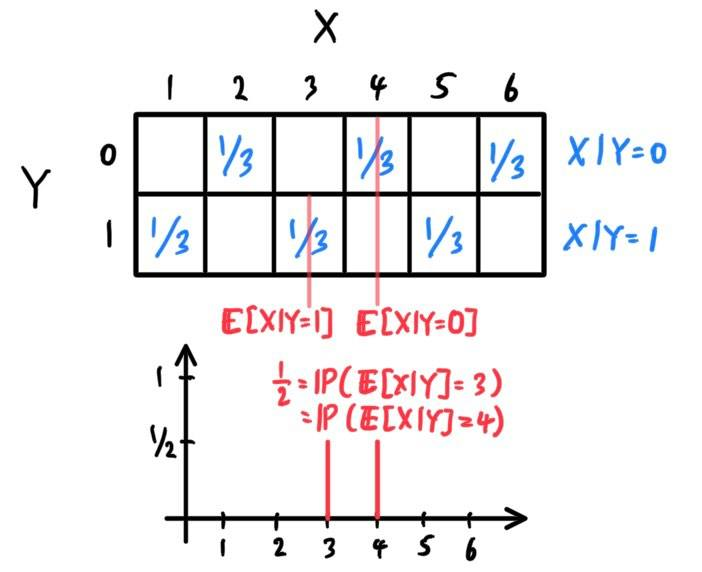
\includegraphics[scale=0.3]{img/conditional_expect_dice.jpg}
    \end{center}
  \end{enumerate}

  From the visual above, we can see that we take the joint distribution $X \times Y$, and for each value $Y = y$, we can estimate $X$ as $\mathbb{E}[X \mid Y = y]$. But now there is the additional uncertainty of what value $Y$ will take, which turns this value estimate $\mathbb{E}[X \mid Y = y]$ in a distribution $\mathbb{E}[X \mid Y]$. So, for the discrete case, 
  \begin{equation}
    \mathbb{P}\big( \mathbb{E}[X \mid Y] = \mathbb{E}[X \mid Y = y]) = \mathbb{P}(Y = y)
  \end{equation}

  Now we can talk about how to compute conditional expectation. In essence, the conditional expectation $\mathbb{E}[X \mid Y]$ is simply a function of a random variable $Y$ that is this best approximation. Given a joint random variable $(X, Y): \Omega \rightarrow \mathbb{R}^2$, we can fix a value of $Y = y$. Therefore, we are given the information that event $Y^{-1}(\{y\})$ happened, and so we can construct our conditional distribution $X \mid Y = y$, which defines a new probability measure. Taking the expectation of that gives us a number. 


  \begin{definition}[Discrete Conditional Expectation Given $Y = y$]
    \label{def:discrete-conditional-expectation-given-yy}
    Let $X: \Omega \to \mathcal{X}$ and $Y: \Omega \to \mathcal{Y}$ be \hyperref[def:discrete-random-variable]{discrete random variables}, and let $y \in \mathcal{Y}$ be such that $\mathbb{P}(Y = y) > 0$. Recall that the \hyperref[def:conditional-pmf]{conditional PMF} is 
    \begin{equation}
      \mathbb{P}(X = x \mid Y = y) \coloneqq \frac{\mathbb{P}(X = x, Y = y)}{\mathbb{P}(Y = y)}
    \end{equation}
    The \textbf{conditional expectation} of $X$ given $Y = y$ is 
    \begin{equation}
      \mathbb{E}[X \mid Y = y] = \sum_{x \in \mathcal{X}} x \, \mathbb{P}(X = x \mid Y = y)
    \end{equation}
  \end{definition}

  \begin{definition}[Continuous Conditional Expectation Given $Y = y$]
    \label{def:continuous-conditional-expectation-given-yy}
    Let $X, Y$ be jointly continuous with joint PDF $f_{X, Y} (x, y)$. Recall that for $y$ such that $f_Y (y) > 0$, the conditional PDF is 
    \begin{equation}
      f_{X \mid Y} (x \mid y) \coloneqq \frac{f_{X, Y} (x, y)}{f_Y (y)}
    \end{equation}
    The \textbf{conditional expectation} of $X$ given $Y = y$ is 
    \begin{equation}
      \mathbb{E}[X \mid Y = y] = \int_{x \in \mathbb{R}} x \, f_{X \mid Y} (x \mid y) \, dx
    \end{equation}
    Again, we can set $\psi(y) \coloneqq \mathbb{E}[X \mid Y = y]$, which is a function of $y$ and therefore a \hyperref[def:random-variable]{random variable}. 
  \end{definition}

  As a visual, we can take a "slice" of the joint distribution of some value of $Y$, look at the distribution of $X$ on this slice, and compute its expectation. That is, for every value of $Y = y$, there exists some (conditional) distribution of $X$ with PMF of $p_{X \mid Y} (x \mid y)$ or PDF of $f_{X \mid Y} (x \mid y)$. 
  \begin{center}
    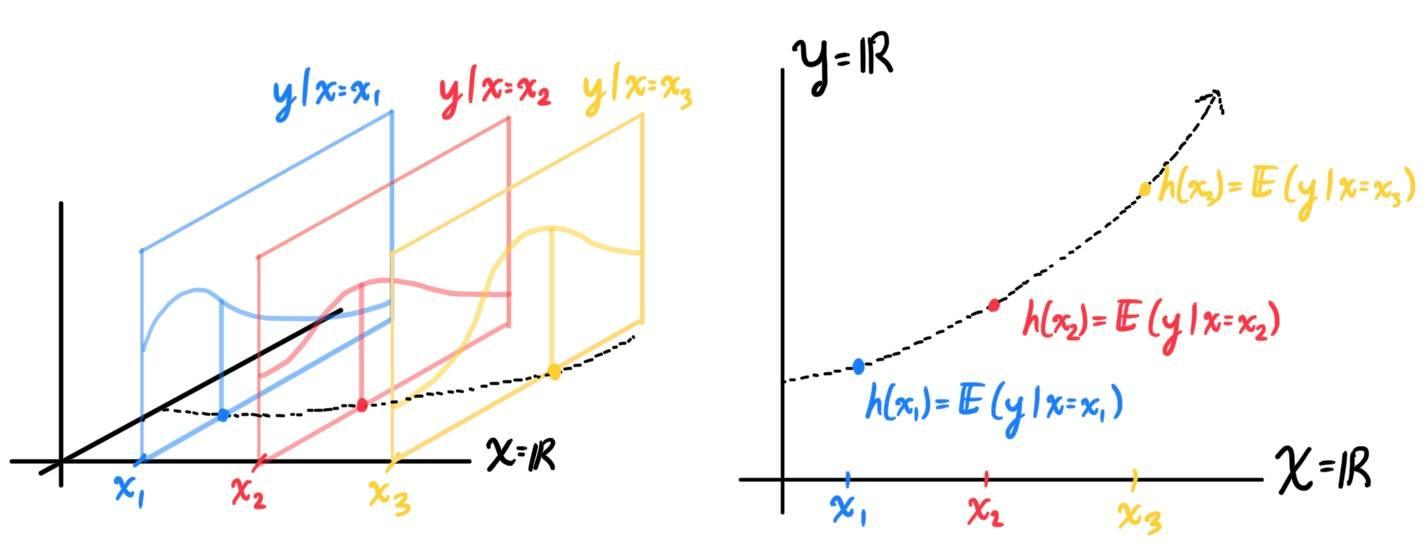
\includegraphics[scale=0.3]{img/conditional_exp.jpg}
  \end{center}
  So given a value of $Y = y$, we generally know something about $X$ (e.g. if I know humidity, I know something about the temperature) and want to find the best estimate of $X$. This is precisely the \hyperref[def:cond-exp]{conditional expectation} $\mathbb{E}[X \mid Y = y]$, and we can interpret this as a regression function $\psi(y) \coloneqq \mathbb{E}[X \mid Y = y]$, which predicts the expected value of $X$ given $Y = y$. 

  But since we don't know what exactly $Y$ is, this process is random itself, and it is only after this $Y$ is realized that we can provide the expected value of $X$. Thus, by replacing the little $y$'s with the big $Y$'s, we can construct a \hyperref[def:random-variable]{random variable} that will estimate $X$ for us given $Y$, denoted $\mathbb{E}[X \mid Y] = \psi(Y)$. This turns out to be a $\sigma(Y)$-measurable random variable itself. 

  \begin{example}[Computing $\mathbb{E}[Y \mid X]$ from a Joint Density]
    \label{ex:find-first-calculate-marginal-density}
    Let $f_{X, Y} (x, y) = \frac{1}{x}$ for $0 < y \leq x \leq 1$. Find $\mathbb{E}[Y \mid X]$. We first calculate the marginal density of $X$, which will allow us to calculate the conditional density of $Y$: 
    \begin{equation}
      f_X (x) = \int_0^x \frac{1}{x} \,dy = \frac{y}{x} \bigg|_0^x = 1 \implies f_{Y \mid X} (y \mid x) = \frac{f_{X, Y} (x, y)}{f_X (x)} = \frac{1/x}{1} = \frac{1}{x} \text{ for } 0 < y \leq x \leq 1
    \end{equation}
    Since the conditional density of $Y$ is not dependent on $x$, $Y$ is uniform from $0$ to $x$. Now calculate the expectation: 
    \begin{equation}
      \mathbb{E}[Y \mid X = x] = \int_0^x y \cdot \frac{1}{x} \,dy = \frac{x}{2}
    \end{equation}
    and so the \hyperref[def:cond-exp]{conditional expectation} is 
    \begin{equation}
      \mathbb{E}[Y \mid X] = \frac{1}{2} X
    \end{equation}
  \end{example}

  \begin{theorem}[Conditional Distribution of a Standard Bivariate Gaussian]
    \label{thm:conditional-distribution-of-a-standard-bivariate-gaussian}
    Let $(X, Y)$ be a \hyperref[thm:marginals-of-a-standard-bivariate-gaussian]{standard bivariate Gaussian} with correlation $\rho$, $|\rho| < 1$. 
    \begin{enumerate}
      \item The conditional distribution of $X$ given $Y = y$ is $X \mid Y = y \sim \mathcal{N} (\rho y, 1 - \rho^2)$. That is, 
      \begin{equation}
        f_{X \mid Y} (x \mid y) = \frac{1}{\sqrt{2 \pi (1 - \rho^2)}} \, \exp\bigg( - \frac{(x - \rho y)^2}{2 (1 - \rho^2)} \bigg)
      \end{equation}
      \item $\mathbb{E}[X \mid Y = y] = \rho y$, and so the conditional expectation of $X$ given $Y$ (which is a \hyperref[def:random-variable]{random variable}) is 
      \begin{equation}
        \mathbb{E}[X \mid Y] = \rho Y
      \end{equation}
      i.e. $\mathbb{E}[X \mid Y]$ is a linear function of $Y$. 
    \end{enumerate}
  \end{theorem}
  \begin{proof}
    (1) By the marginal computation, $f_Y (y) = e^{-y^2/2} / \sqrt{2 \pi}$, so 
    \begin{equation}
      f_{X \mid Y} (x \mid y) = \frac{f_{X, Y} (x, y)}{f_Y (y)} = \frac{1}{\sqrt{2 \pi} \sqrt{1 - \rho^2}} \exp \bigg( -\frac{x^2 - 2 \rho x y + y^2 - (1 - \rho^2) y^2}{2 (1 - \rho^2)} \bigg)
    \end{equation}
    and since $x^2 - 2 \rho x y + \rho^2 y^2 = (x - \rho y)^2$, this is the stated PDF. 

    (2) The mean of $\mathcal{N}(\rho y, 1 - \rho^2)$ is $\rho y$, and $\psi(y) = \rho y$ gives $\mathbb{E}[X \mid Y] = \psi(Y) = \rho Y$. 
  \end{proof}

  A fundamental result in statistical learning theory is that if we have two \hyperref[def:random-variable]{random variables} $X$ and $Y$, the best predictor of $Y$ as a function of $X$ is the \hyperref[def:cond-exp]{conditional expectation} $\mathbb{E}[Y \mid X]$. 

  \begin{theorem}[Conditional Expectation as the $L^2$ Projection]
    \label{thm:two-random-variables-function-minimizes}
    Let us have two \hyperref[def:random-variable]{random variables} $X$ and $Y$, with $g(X) = \mathbb{E}[Y \mid X]$. Then, the function $g$ minimizes the cost function $\mathbb{E}[ (Y - h(X))^2]$. That is, 
    \begin{equation}
      \inf_{h \text{ meas.}} \mathbb{E}[( Y - h(X))^2] = \mathbb{E} [(Y - g(X))^2]
    \end{equation}
  \end{theorem}

	\begin{example}[Fair Coin Toss Game]
	  \label{ex:fair-coin-toss-game}
		Alice and Bob each choose a random number uniformly between $0$ and $1$. After Alice chooses her number, she has the option to redraw. At the end, whoever has the greater number wins. What is the probability that Alice wins? 

		Let $A$ and $B$ be the \hyperref[def:random-variable]{random variables} representing Alice and Bob's final draw. Let $S \sim \Bernoulli(p)$ be the random variable representing whether Alice redraws ($S = 1$) or stays ($S = 0$). Then, by the \hyperref[thm:tower-rule]{tower rule}, 
		\begin{align}
			\mathbb{E}[A] & = \mathbb{E}[\mathbb{E}[A \mid S]] \\ 
										& = \mathbb{E}[A \mid S = 0] \mathbb{P}(S = 0) + \mathbb{E}[A \mid S = 1] \mathbb{P}(S = 1) \\ 
										& = \frac{1 + p}{2} (1 - p) + \frac{1}{2} p
		\end{align}
		which has a maximum at $p = \frac{1}{2}$ with a value of $\frac{5}{8}$. 
	\end{example}

	We can also use recursion to solve for expectation. 

	\begin{example}[Expected Number of Rolls Before Getting Two 6s in a Row]
	  \label{ex:expected-number-of-rolls-before-getting-two-6s}
		You have a fair dice. What is the expected number of rolls before you get two 6s in a row? 

		Let $X_{66}$ be the \hyperref[def:random-variable]{random variable} that represents how many dice rolls we have before we get a $6$. The intuitive thing is to condition it on whether we get a 6 on our first dice roll. Therefore, let $Y_1, Y_2$ be our first and second dice rolls. By the tower property, 
		\begin{align}
			\mathbb{E}[X_{66}] & = \mathbb{E}[ \mathbb{E}[X_{66} \mid Y_1]] \\ 
												 & = \mathbb{E}[X_{66} \mid Y_1 = 0] \mathbb{P}(Y_1 = 0) + \mathbb{E}[X_{66} \mid Y_1 = 1] \mathbb{P}(Y_1 = 1) \\ 
												 & = \frac{5}{6} (1 + \mathbb{E}[X_66]) + \frac{1}{6} (1 + \mathbb{E}[X_{66} \mid Y_1 = 1])
		\end{align}
		Note that $Z = X_{66} \mid Y_1 = 1$ is the \textit{additional} dice rolls after you roll the $6$, and we also have two cases for this. 
		\begin{align}
			\mathbb{E}[Z] & = \mathbb{E}[\mathbb{E}[Z \mid Y_2]] \\ 
										& = \mathbb{E}[Z \mid Y_2 = 0] \mathbb{P}(Y_2 = 0) + \mathbb{E}[Z \mid Y_2 = 1] \mathbb{P}(Y_2 = 1) \\ 
										& = (1 + \mathbb{E}[X_{66}]) \frac{5}{6} + \frac{1}{6} (1)
		\end{align}
		Solving the system of two linear equations gives $\mathbb{E}[X_{66}] = 42$. 
	\end{example}

	\begin{example}[Expected Number of Rolls Before Getting 6 Followed by a 5]
	  \label{ex:expected-number-of-rolls-before-getting-6}
		
	\end{example}

	\begin{example}[Expected Number of Flips to Get 10 Heads in a Row]
	  \label{ex:expected-number-of-flips-to-get-10-heads-in-a}
		We first condition on the first coin flip $Z_1$. 
		\begin{align}
			\mathbb{E}[X_{10}] & = \mathbb{E}[\mathbb{E}[X_{10} \mid Z_1]] \\ 
												 & = \mathbb{E}[X_{10} \mid Z_1 = 0] \mathbb{P}(Z_1 = 0) + \mathbb{E}[X_{10} \mid Z_1 = 1] \mathbb{P}(Z_1 = 1) \\ 
												 & = \frac{1}{2} (1 + \mathbb{E}[X_{10}]) + \frac{1}{2} (1 + \mathbb{E}[X_9]) \\ 
												 & = 1 + \frac{1}{2} \mathbb{E}[X_{10}] + \frac{1}{2} \mathbb{E}[X_9] 
		\end{align}
		Let $Z_2$ be the next coin flip after getting a heads. Then, we can condition again $Z_2$. 
		\begin{align}
			\mathbb{E}[X_{9}]  & = \mathbb{E}[\mathbb{E}[X_{9} \mid Z_2]] \\ 
												 & = \mathbb{E}[X_{9} \mid Z_2 = 0] \mathbb{P}(Z_2 = 0) + \mathbb{E}[X_{9} \mid Z_2 = 1] \mathbb{P}(Z_2 = 1) \\ 
												 & = \frac{1}{2} (1 + \mathbb{E}[X_{10}]) + \frac{1}{2} (1 + \mathbb{E}[X_8]) \\ 
												 & = 1 + \frac{1}{2} \mathbb{E}[X_{10}] + \frac{1}{2} \mathbb{E}[X_8] 
		\end{align}
		and we can keep doing this until we reach 
		\begin{equation}
			\mathbb{E}[X_1] = 1 + \frac{1}{2} \mathbb{E}[X_{10}]
		\end{equation}
		Solving this system of 10 equations gives $\mathbb{E}[X_{10}] = 2046$. 
	\end{example}

  \begin{example}[Expectation of a Random Sum]
    \label{ex:random-sum-random-variables-iid}
    Consider the random sum of \hyperref[def:random-variable]{random variables} $S_N = \sum_{i=1}^N X_i$, where $X_i$ are iid and $N$ is independent of $X_i$'s. Then, we can use the \hyperref[thm:tower-rule]{tower rule} to write $\mathbb{E}[S_N] = \mathbb{E}[\mathbb{E}[S_N \mid N]]$. $\mathbb{E}[S_N \mid N]$ is a transformed random varibale of $N$, and to compute its closed form we should just compute $\mathbb{E}[S_N \mid N = n]$ and replace $n$ with $N$. 
    \begin{equation}
      \mathbb{E}[S_N \mid N = n] = \mathbb{E}[S_n] = \mathbb{E} \bigg( \sum_{i=1}^n X_i \bigg) = n \mathbb{E}[X]
    \end{equation}
    remember that $\mathbb{E}[X]$ is just a number, so replacing $n$ with $N$ gives $\mathbb{E}[S_N \mid N] = N \mathbb{E}[X]$, i.e. the random variable $N$ multiplied by $\mathbb{E}[X]$. Therefore, 
    \begin{equation}
      \mathbb{E}[\mathbb{E}[S_N \mid N]] = \mathbb{E}[N \mathbb{E}[X]] = \mathbb{E}[N] \, \mathbb{E}[X]
    \end{equation}
    This makes sense intuitively, since we want to approximate this value by taking the expected value of $X$ and multiplying it by the expected number of summands. 
  \end{example}

  Now, we can simply use the property to talk about what $\mathbb{P}(X \mid Y)$ means. Formally, using the fact that the probability that $X$ will realize in $A$, i.e. $\mathbb{P}(X \in A) = \mathbb{E}_X[1_A]$, we can define the conditional probability as 
  \begin{equation}
    \mathbb{P}(X \in A \mid Y) = \mathbb{E}[ 1_X \mid Y]
  \end{equation}
  We can interpret this in multiple ways, in increasing level of rigor. Let $(\Omega, \mathcal{F}, \mathbb{P})$ be a \hyperref[def:probability-space]{probability space}, with \hyperref[def:random-variable]{random variables} $X, Y$ with their probability laws $\mathbb{P}_X, \mathbb{P}_Y$. 
  \begin{enumerate}
    \item When $Y$ realizes, we can use this definition to have a better educated guess of where $X$ will land. But since $Y$ is random, so is our guess. 
    
    \item Let us have the joint distribution $(X, Y)$. Given that $Y = y$, we can take the conditional distribution $X \mid Y = y$ and compute the event that this random variable lands in $A$ by replacing the little $y$'s with the big $Y$'s. 
    
    \item Let $A$ be an event in $\mathcal{R}$. Then, the probability that $X$ will land in $A$ is 
    \begin{equation}
      \mathbb{P}(X \in A) = \mathbb{P}_X(A) = \mathbb{P}(X^{-1} (A))
    \end{equation}
    where the first is shorthand for the second, which is the probability law on $\mathbb{R}$, and the third is the probability law on $\Omega$. Then, $1_A$ generates a $\sigma$-algebra $\sigma(1_A)$ on $\Omega$, consisting of the sets $\{\emptyset, X^{-1}(A), X^{-1}(A)^c, \Omega\}$. 
  \end{enumerate}


  Now the $\sigma$-algebra generated by multiple random variables should intuitively be bigger than the $\sigma$-algebra generated by one random variable. We can't simply take the union of the individual $\sigma$-algebras. 

  \begin{definition}[$\sigma$-algebra generated by Multiple Random Variables]
    \label{def:sigma-algebra-generated-by-multiple-random}
    Given random variables $\{X_i\}_{i \in I}$ indexed by some set (possibly uncountable), the $\sigma$-algebra generated by this collection is defined 
    \begin{equation}
      \sigma(X_1, \ldots, X_n) \coloneqq \sigma \bigg( \bigcup_{i \in I} \sigma(X_i) \bigg)
    \end{equation}
  \end{definition}

  Let us look at $\mathbb{E}[X \mid Y, Z]$ and compare it to $\mathbb{E}[X \mid Y]$. From this definition, we know that the information about $X$ contained in $\sigma(Y, Z)$ is at least as great as the corresponding information in $\sigma(Y)$. Therefore, we can simply define \hyperref[def:cond-exp]{conditional expectation} as such: 

  \begin{definition}[Conditional Expectation given Multiple Random Variables]
    \label{def:conditional-expectation-given-multiple-random}
    Given \hyperref[def:random-variable]{random variables} $\{X_i\}_{i \in I}$, the \hyperref[def:cond-exp]{conditional expectation} is defined 
    \begin{equation}
      \mathbb{E}[Y \mid \{X_i\}_{i \in I} ] = \mathbb{E}[ Y \mid \sigma(\{X_i \}_{i \in I}]
    \end{equation}
    which is the random variable where 
    \begin{equation}
      \int_A Y \, d\mathbb{P} = \int_A \mathbb{E}[Y \mid \{X_i\}_{i \in I} ] \, d\mathbb{P}
    \end{equation}
    for all $A \in \sigma(\{X_i \}_{i \in I})$. 
  \end{definition}

\subsection{Conditional Variance}

  Similar to \hyperref[def:cond-exp]{conditional expectation}, we can define the conditional variance $\mathrm{Var}(Y \mid X = x)$ as a function $h(x)$ that outputs the variance of $Y$ given $X = x$. We have
  \begin{align}
    \mathrm{Var}(Y \mid X = x) & = \mathbb{E}\big[ ( Y - \mathbb{E}[Y \mid X = x] )^2 \mid X = x \big]
  \end{align}

  \begin{definition}[Conditional Variance]
    \label{def:conditional-variance}
    The \textbf{conditional variance} of $Y$ given $X$ is defined as 
    \begin{equation}
      \Var(Y \mid X) = \mathbb{E} \big[ \big( Y - \mathbb{E}[Y \mid X] \big)^2 \mid X \big]
    \end{equation}
    which tells us how much variance is left if we use $\mathbb{E}[Y \mid X]$ to predict $Y$. 
  \end{definition}

